\chapter{Piante e sollecitazioni}

\section{Azioni}
\clearpage	
\begin{landscape}
\subsection{SLU}
\begin{figure}[H]
\centering
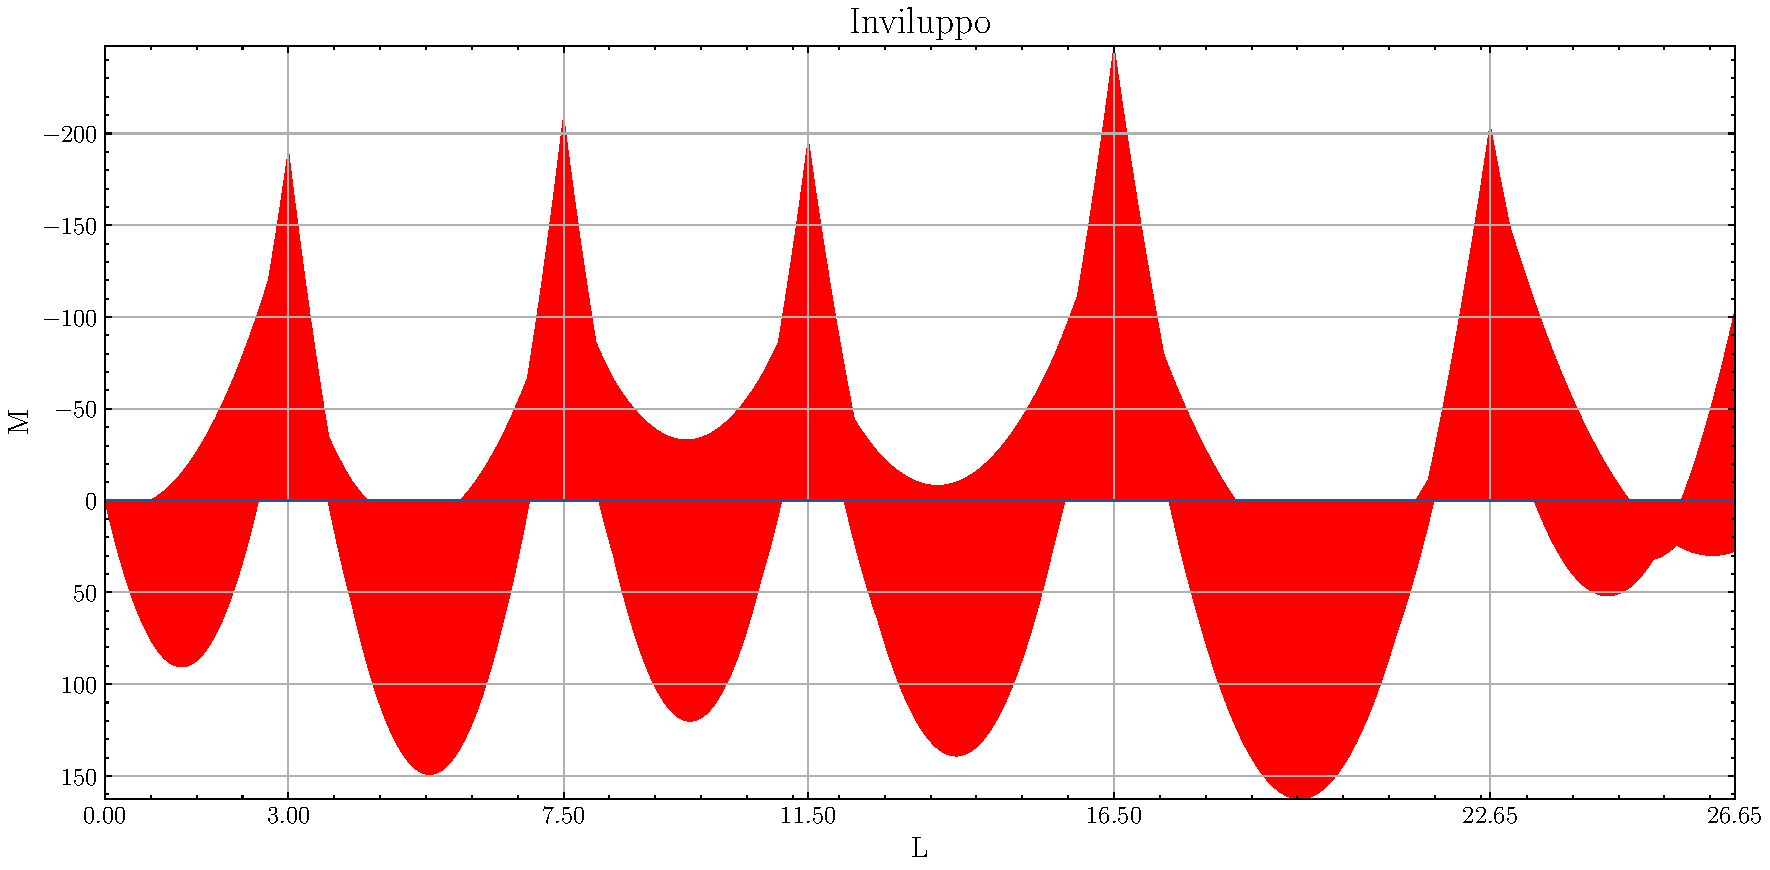
\includegraphics[height=0.6\textwidth]{IMG/diagrammi_trave/m.pdf}
\caption{Diagrammi del momento generati con combinazione di carico SLU}
\label{fig:trave_ULS_momento}
\end{figure}
\begin{table}[H]
\footnotesize
\centering
\caption{Valori del momento con combinazione di carico SLU nei punti più significativi della struttura}
\label{tab:trave_ULS_momento}
	\begin{tabular}{lS[table-format=-3.2]S[table-format=-3.2]S[table-format=-3.2]S[table-format=-3.2]S[table-format=-3.2]S[table-format=-3.2]S[table-format=-3.2]S[table-format=-3.2]S[table-format=-3.2]S[table-format=-3.2]S[table-format=-3.2]S[table-format=-3.2]S[table-format=-3.2]}
		\toprule
		{} & {A1} & {C1} & {A2} & {C2} & {A3} & {C3} & {A4} & {C4} & {A5} & {C5} & {A6} & {C6} & {A7} \\
		\midrule
		$s\,\si{[\metre]}$ & 0.00 & 1.26 & 3.00 & 5.31 & 7.50 & 9.57 & 11.50 & 13.92 & 16.50 & 19.54 & 22.65 & 24.57 & 26.65 \\
        $M^{-}\,\si{[\kilo\newton\metre]}$ & 0.00 & -15.14 & -190.97 & 0.00 & -209.46 & -33.15 & -196.60 & -10.06 & -247.45 & 0.00 & -204.82 & -18.04 & -103.04 \\
        $M^{+}\,\si{[\kilo\newton\metre]}$ & 0.00 & 90.60 & 0.00 & 149.18 & 0.00 & 120.20 & 0.00 & 139.16 & 0.00 & 162.53 & 0.00 & 51.88 & 27.68 \\
		\bottomrule
	\end{tabular}
\end{table}
\end{landscape}

%{} & {A1} & {C1} & {A2} & {C2} & {A3} & {C3} & {A4} & {C4} & {A5} & {C5} & {A6} & {C6} & {A7} \\
%&\multicolumn{1}{c}{Nodo 1}&\multicolumn{1}{c}{Camp. 1}&\multicolumn{1}{c}{Nodo 2}&\multicolumn{1}{c}{Camp. 2}&\multicolumn{1}{c}{Nodo 3}&\multicolumn{1}{c}{Camp. 3}&\multicolumn{1}{c}{Nodo 4}&\multicolumn{1}{c}{Camp. 4}&\multicolumn{1}{c}{Nodo 5}&\multicolumn{1}{c}{Camp. 5}&\multicolumn{1}{c}{Nodo 6}&\multicolumn{1}{c}{Camp. 6}&\multicolumn{1}{c}{Nodo 7}\\
		
